% Options for packages loaded elsewhere
\PassOptionsToPackage{unicode}{hyperref}
\PassOptionsToPackage{hyphens}{url}
%
\documentclass[
]{article}
\usepackage{amsmath,amssymb}
\usepackage{iftex}
\ifPDFTeX
  \usepackage[T1]{fontenc}
  \usepackage[utf8]{inputenc}
  \usepackage{textcomp} % provide euro and other symbols
\else % if luatex or xetex
  \usepackage{unicode-math} % this also loads fontspec
  \defaultfontfeatures{Scale=MatchLowercase}
  \defaultfontfeatures[\rmfamily]{Ligatures=TeX,Scale=1}
\fi
\usepackage{lmodern}
\ifPDFTeX\else
  % xetex/luatex font selection
\fi
% Use upquote if available, for straight quotes in verbatim environments
\IfFileExists{upquote.sty}{\usepackage{upquote}}{}
\IfFileExists{microtype.sty}{% use microtype if available
  \usepackage[]{microtype}
  \UseMicrotypeSet[protrusion]{basicmath} % disable protrusion for tt fonts
}{}
\makeatletter
\@ifundefined{KOMAClassName}{% if non-KOMA class
  \IfFileExists{parskip.sty}{%
    \usepackage{parskip}
  }{% else
    \setlength{\parindent}{0pt}
    \setlength{\parskip}{6pt plus 2pt minus 1pt}}
}{% if KOMA class
  \KOMAoptions{parskip=half}}
\makeatother
\usepackage{xcolor}
\usepackage[margin=1in]{geometry}
\usepackage{graphicx}
\makeatletter
\def\maxwidth{\ifdim\Gin@nat@width>\linewidth\linewidth\else\Gin@nat@width\fi}
\def\maxheight{\ifdim\Gin@nat@height>\textheight\textheight\else\Gin@nat@height\fi}
\makeatother
% Scale images if necessary, so that they will not overflow the page
% margins by default, and it is still possible to overwrite the defaults
% using explicit options in \includegraphics[width, height, ...]{}
\setkeys{Gin}{width=\maxwidth,height=\maxheight,keepaspectratio}
% Set default figure placement to htbp
\makeatletter
\def\fps@figure{htbp}
\makeatother
\setlength{\emergencystretch}{3em} % prevent overfull lines
\providecommand{\tightlist}{%
  \setlength{\itemsep}{0pt}\setlength{\parskip}{0pt}}
\setcounter{secnumdepth}{-\maxdimen} % remove section numbering
\ifLuaTeX
  \usepackage{selnolig}  % disable illegal ligatures
\fi
\usepackage{bookmark}
\IfFileExists{xurl.sty}{\usepackage{xurl}}{} % add URL line breaks if available
\urlstyle{same}
\hypersetup{
  pdftitle={Summer Assignment Overview},
  hidelinks,
  pdfcreator={LaTeX via pandoc}}

\title{Summer Assignment Overview}
\author{}
\date{\vspace{-2.5em}}

\begin{document}
\maketitle

\begin{figure}
\centering

\includegraphics{figs/logo.png}
\caption{Kennedy School Logo}
\end{figure}

Welcome to the Summer 2024 Pre-Assignment! This readme file will provide
you with the basic structure of the folder in Posit Cloud and an
overview of what tools and resources we will be using.

\subsection{Folder Structure}\label{folder-structure}

In your Posit Cloud workspace, you will find the following folder
structure:

\begin{verbatim}
/summer-assignment
  ├── assignments
      ├── R Summer Assignment 1.rmd
      ├── R Summer Assignment 2.rmd
      ├── R Summer Assignment 3.rmd
      └── R Summer Assignment 4.rmd
      └── R Summer Assignment 5.rmd
\end{verbatim}

\subsubsection{/assignments}\label{assignments}

This folder contains all the assignments you will need to complete
during the summer. Each assignment is provided as a RMarkdown
(\texttt{.rmd}) file. You will be working on these files directly in
Posit Cloud.

\begin{figure}
\centering
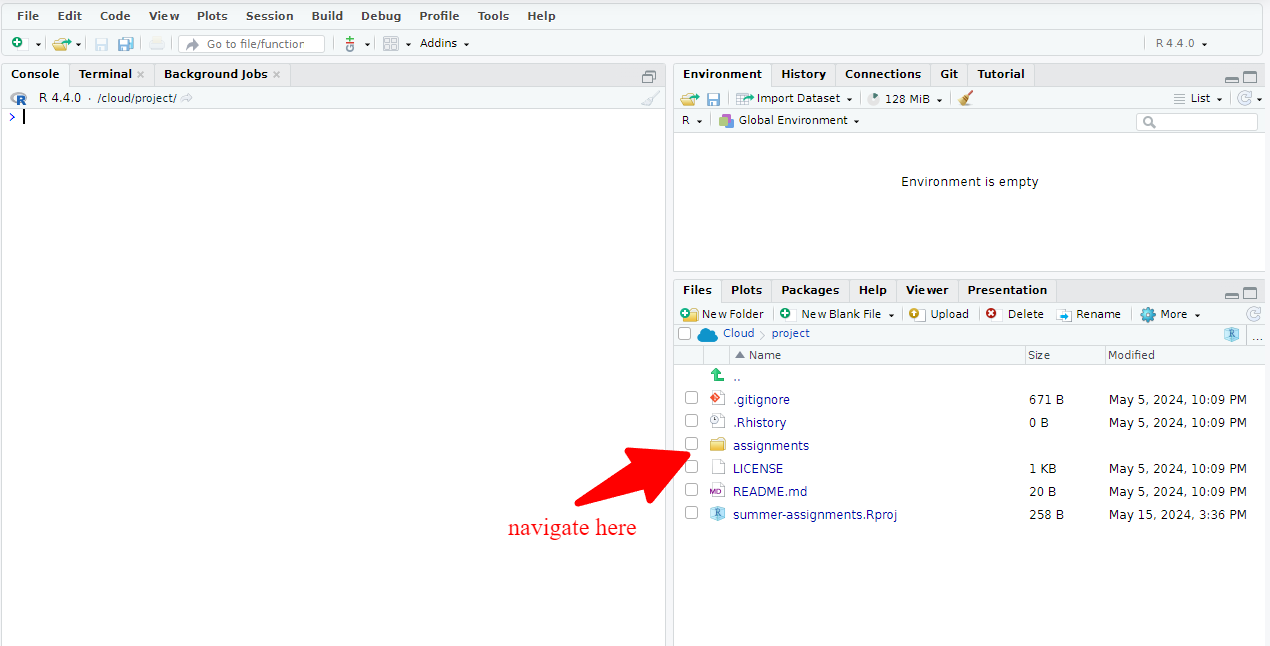
\includegraphics{figs/folder_structure.png}
\caption{Folder Structure}
\end{figure}

\subsection{Tools and Resources}\label{tools-and-resources}

\subsubsection{Posit Cloud}\label{posit-cloud}

We will be using Posit Cloud as our primary platform for completing
assignments. Posit Cloud allows you to write, execute, and save R code
in a cloud environment, making it accessible from any device with an
internet connection.

\subsubsection{R and RStudio}\label{r-and-rstudio}

R is the programming language we will be using for data analysis.
RStudio is an integrated development environment (IDE) for R that
provides a user-friendly interface for writing and running R code.

\subsubsection{GitHub}\label{github}

You will need a GitHub account to manage your projects and collaborate
with others. If you haven't created a GitHub account yet, please do so
before starting the assignments.

\subsubsection{RMarkdown}\label{rmarkdown}

RMarkdown is a powerful tool that combines Markdown and R code to create
dynamic, reproducible documents. You will be using it to write and
execute your R code within the assignments.

\subsection{Submission}\label{submission}

Complete your assignments in the Posit Cloud environment. Please submit
only the \texttt{.rmd} file you are working on to the Assignment Page on
Canvas. We will announce when the Canvas site is created.

\subsection{Help and Support}\label{help-and-support}

If you get stuck or need assistance, please use Slack to ask the
teaching team.

Happy coding!

\end{document}
